\subsection{Dalitzplots}
\label{sec:dalitz-plots}

\begin{figure}[ht!]
  \centering
  \vspace{-0.3cm}
  \subbottom[Dobbeltkoincidenser]{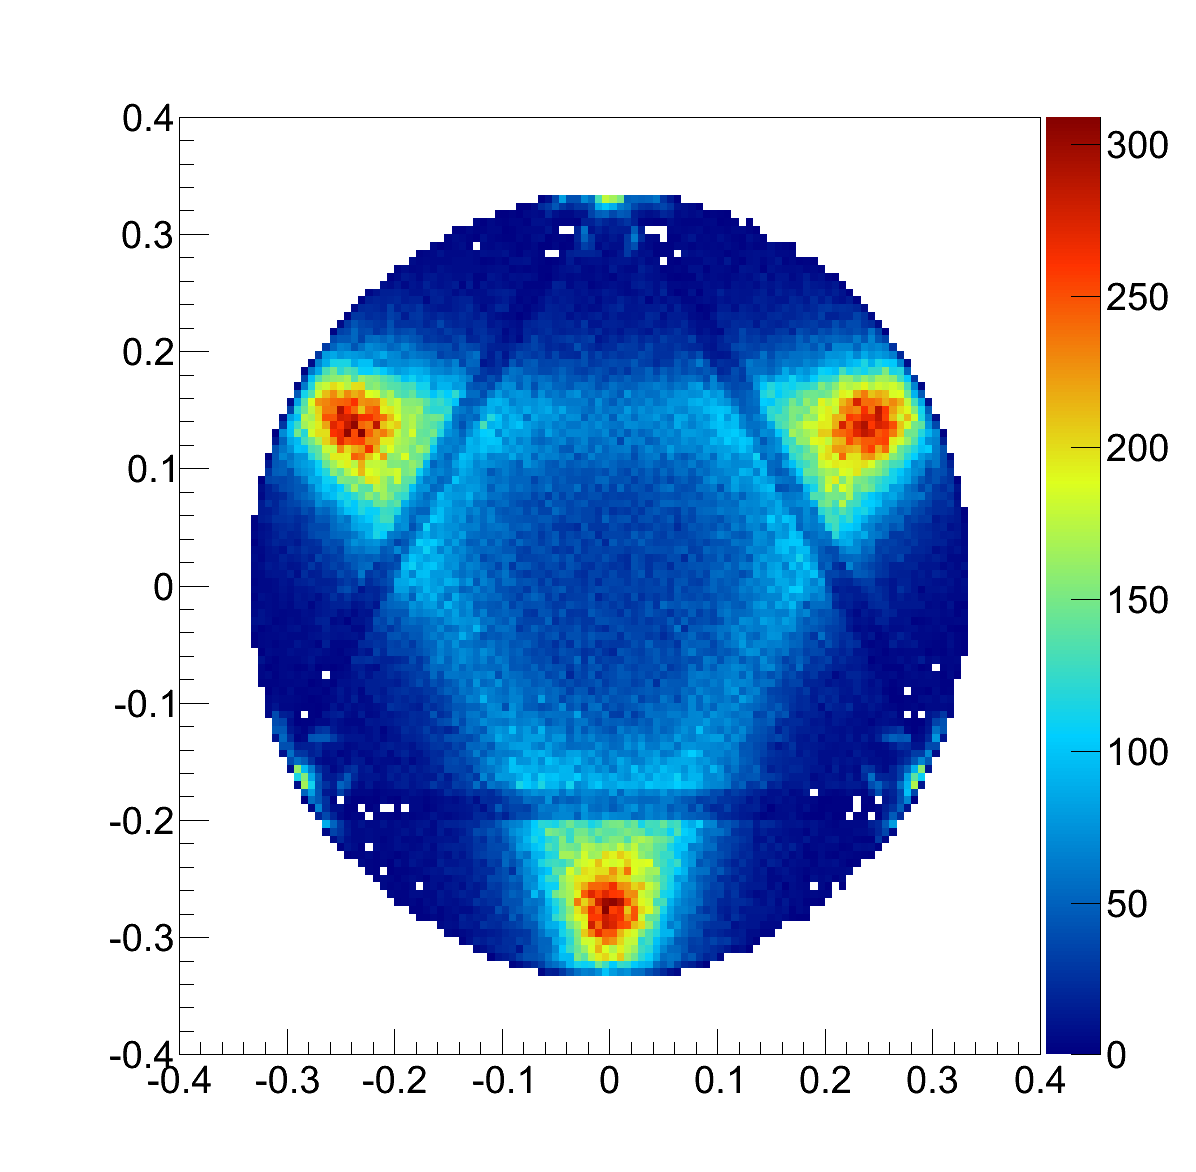
\includegraphics[width=0.42\columnwidth]{1077-Dalitz-D}}%
  \hfill
  \subbottom[Trippelkoincidenser]{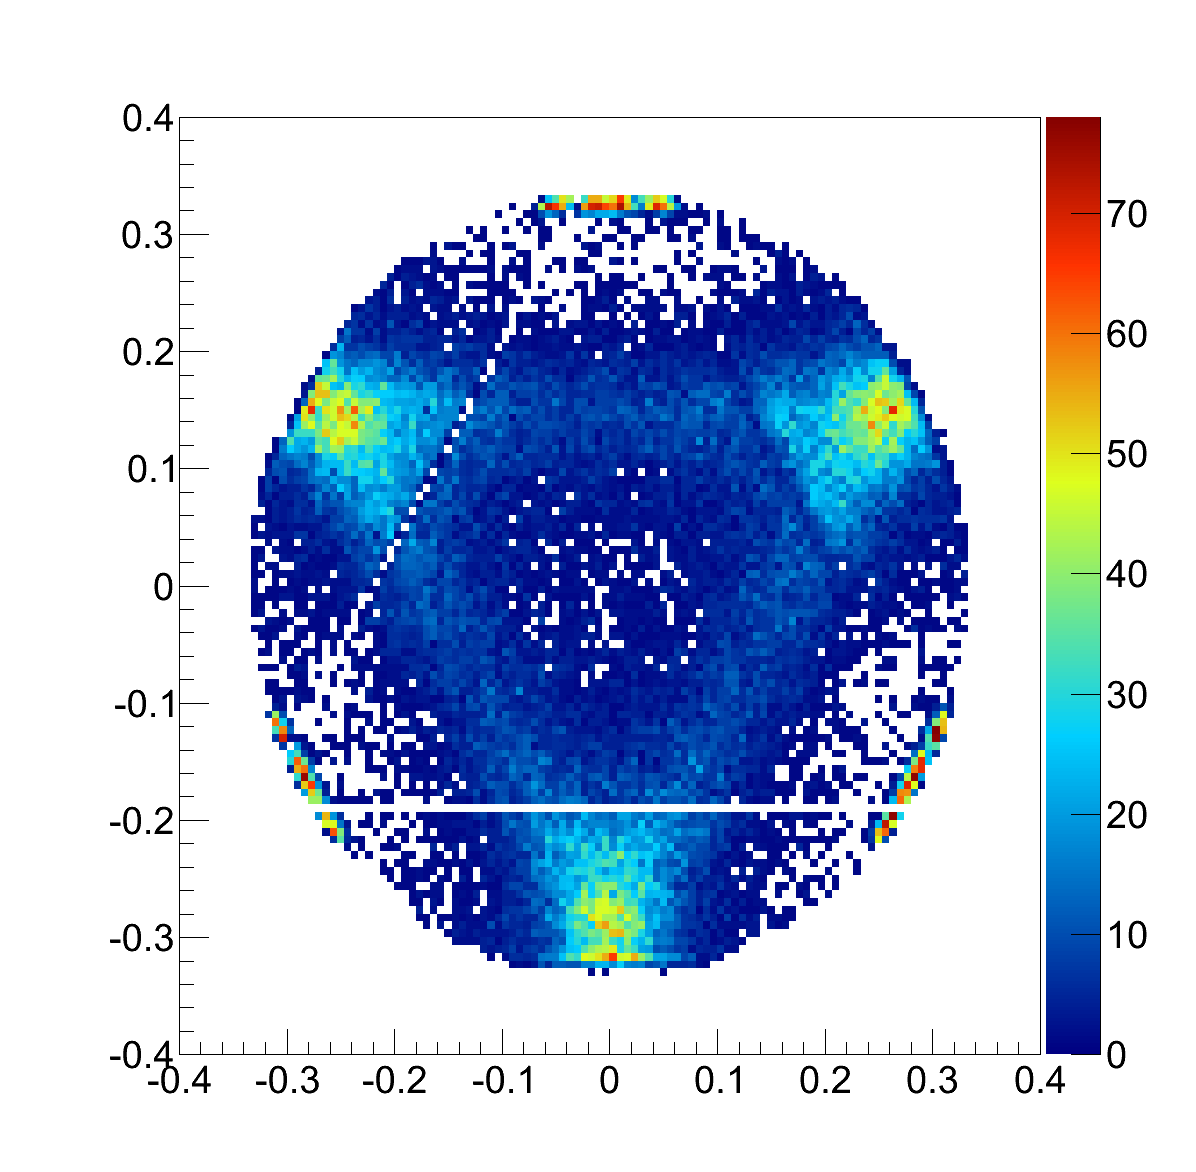
\includegraphics[width=0.42\columnwidth]{1077-Dalitz-T}}%
  \caption{Dalitzplot for $0^{+}$ tilstanden ved \SI{17.8}{\MeV} i kulstof.}
  \label{fig:dalitz-1077}
  % 
  % 
  % 
  \subbottom[Dobbeltkoincidenser]{\includegraphics[width=0.42\columnwidth]{1108-Dalitz-D}}%
  \hfill
  \subbottom[Trippelkoincidenser]{\includegraphics[width=0.42\columnwidth]{1108-Dalitz-T}}%
  \caption{Dalitzplot for $1^{+}$ tilstanden ved \SI{18.2}{\MeV} i kulstof.}
  \label{fig:dalitz-1108}
  % 
  % 
  % 
  \subbottom[Dobbeltkoincidenser]{\includegraphics[width=0.42\columnwidth]{1128-Dalitz-D}}%
  \hfill
  \subbottom[Trippelkoincidenser]{\includegraphics[width=0.42\columnwidth]{1128-Dalitz-T}}%
  \caption{Dalitzplot for $3^{-}$ tilstanden ved \SI{18.5}{\MeV} i kulstof.}
  \label{fig:dalitz-1128}
  \vspace{-1.3cm}
\end{figure}

Dalitzplots for de tre tilstande, hvis spektrum blev fundet i foregående afsnit, ses på figurerne
\ref{fig:dalitz-1077} til \ref{fig:dalitz-1128}. Det bemærkes, at for trippelkoincidenserne af
\SI{18.5}{\MeV} tilstanden er plottet skåret af ved 300 tællinger, da det ellers ikke var muligt at
se de detaljerede stukturer.

For det første ses det tydeligt, at data ikke er konsistent med direkte henfald til tre
$\alpha$-partikler.

Generelt gælder for alle Dalitzplots, at der er tre bånd ude ved kanten af cirklen. Disse
stammer fra de mest energirige partikler i henfaldet (jvf. \cref{fig:dalitz-triangle}) og må derfor
være $\alpha_{0}$, hvilket stemmer overens med bredden af båndet, da grundtilstanden af \Be er meget
smal. Lidt under $\alpha_{0}$ ses små strukturer på \cref{fig:dalitz-1077}a og
\ref{fig:dalitz-1128}a. Strukturerne stammer fra den observerede støj i dobbeltkoincidenserne på
\cref{fig:alpha-spec}a og \ref{fig:alpha-spec}e. Som forventet fra \cref{sec:energispektrum}
forekommer $\alpha_{0}$-båndet også i både \ref{fig:dalitz-1108}a og b, hvilket igen indikerer, at der
ikke kan være tale om en $1^{+}$ tilstand.

Ved lidt lavere energi ses $\alpha_{1}$-båndene. For de to laveste energier har toppene i siderne og 
bunden samme struktur på trods af, at toppene er vanskeligere at skille fra baggrunden i
trippelkoincidensplottet. Der hersker dog ingen tvivl om, at bredden af $\alpha_{1}$-båndet er væsentligt
større end $\alpha_{0}$-båndet samt at bredden af $3^{-}$ tilstanden er større end $0^{+}$
tilstanden. De tre toppe er desuden forbundet af linier, som buer indad, hvor det lader til, at
liniernes krumning stiger med energien.

En fuldstændig forståelse af plottet ville kræve en kvantemekanisk tre-partikel model, hvilket
stadig er et aktivt forskningsområde. Derfor er det ikke muligt at redegøre for plottes udseende ud over
båndstrukturen.


Ser man på \cref{fig:dalitz-1077}a og b, kan man ud fra \cref{fig:dalitz-0} udelukke de to tilstande
med naturlig paritet $1^{-}$ og $3^{-}$, da disse kræver, at der er nulpunkter ved de steder, hvor
$\alpha_{1}$-båndet har maksima. Henfald til grundtilstanden af \Be er desuden forbudt for alle
tilstande med unaturlig paritet, hvorved de også kan udelukkes.

Dermed er antallet af kandidater reduceret til $0^{+}$ og $2^{+}$, for hvilke symmetrien stiller
samme krav, hvilket er konsistent med \cite{States}, der angiver en $2^{+}$. Der er desuden den
mulighed, at det kan være en tilstand, som ikke er tabuleret i \cite{Fedorov}.

En tilsvarende analyse med samme resultat kan udføres for de to andre tilstande. Dette indikerer, at
der ikke findes en $1^{+}$ tilstand med isospin 0, da denne ville dominere i forhold til de
omkringliggende isospin 1 tilstande. 

Ifølge \cite{States} er tilstanden ved \SI{18.5}{\MeV} en $3^{-}$ tilstand, hvilket ikke stemmer
overens med denne analyse. Ser man på plottet af trippelkoincidenserne for denne, ses der
uregelmæssigheder ved cirkelranden i området omkring $\alpha_{1}$-båndet. Dette kan skyldes
bagvedliggende tilstande og i mindre grad usikkerheder i placeringen af detektorerne og
kalibreringen. Det er derfor nødvendigt at foretage yderligere analyse, før dette spørgsmål kan
afgøres.

% En videre analyse vil kræve simuleringer, hvilket er uden for tidsrammen af dette
% projekt. Heldigvis er tilstanden tabuleret og ifølge \cite{States} er den populerede tilstand en
% $0^{+}$ tilstand, hvilket stemmer smukt overens med resultaterne.














